

\section{EVALUATION AND RESULTS}
\label{chap:evalution}

\subsection{Evaluation Methods}

The evaluation process is conducted through two main metrics: Mean Opinion Scores (MOS) and Fréchet Inception Distance (FID).

\subsubsection{Evaluation Based on Human Perception}

\textbf{Mean Opinion Scores (MOS)}

Currently, there is no standard metric for gesture generation, especially for gesture generation from speech. Therefore, this paper relies on subjective human evaluation to conduct experimental assessments. 
Similar to previous methods \cite{yoon2022genea}, \cite{kucherenko2021large}, speech-driven gesture generation models still lack objective metrics that consistently reflect human subjective perception \cite{alexanderson2022listen}.

MOS is measured through three criteria:

\begin{itemize}
	\item Human-likeness
	\item Gesture-Speech Appropriateness
	\item Gesture-Style Appropriateness
\end{itemize}

One of the contributions of this paper is the development of the \hyperlink{https://genea-workshop.github.io/leaderboard/}{GENEA Leaderboard} \footnote{ \url{https://genea-workshop.github.io/leaderboard} } \cite{nagy2024towards}. This system includes HEMVIP (\textbf{H}uman \textbf{E}valuation of \textbf{M}ultiple \textbf{V}ideos in \textbf{P}arallel), which is used to compare visual generation results between videos rendered by different models.

%\begin{figure}[h]
%	\centering
%	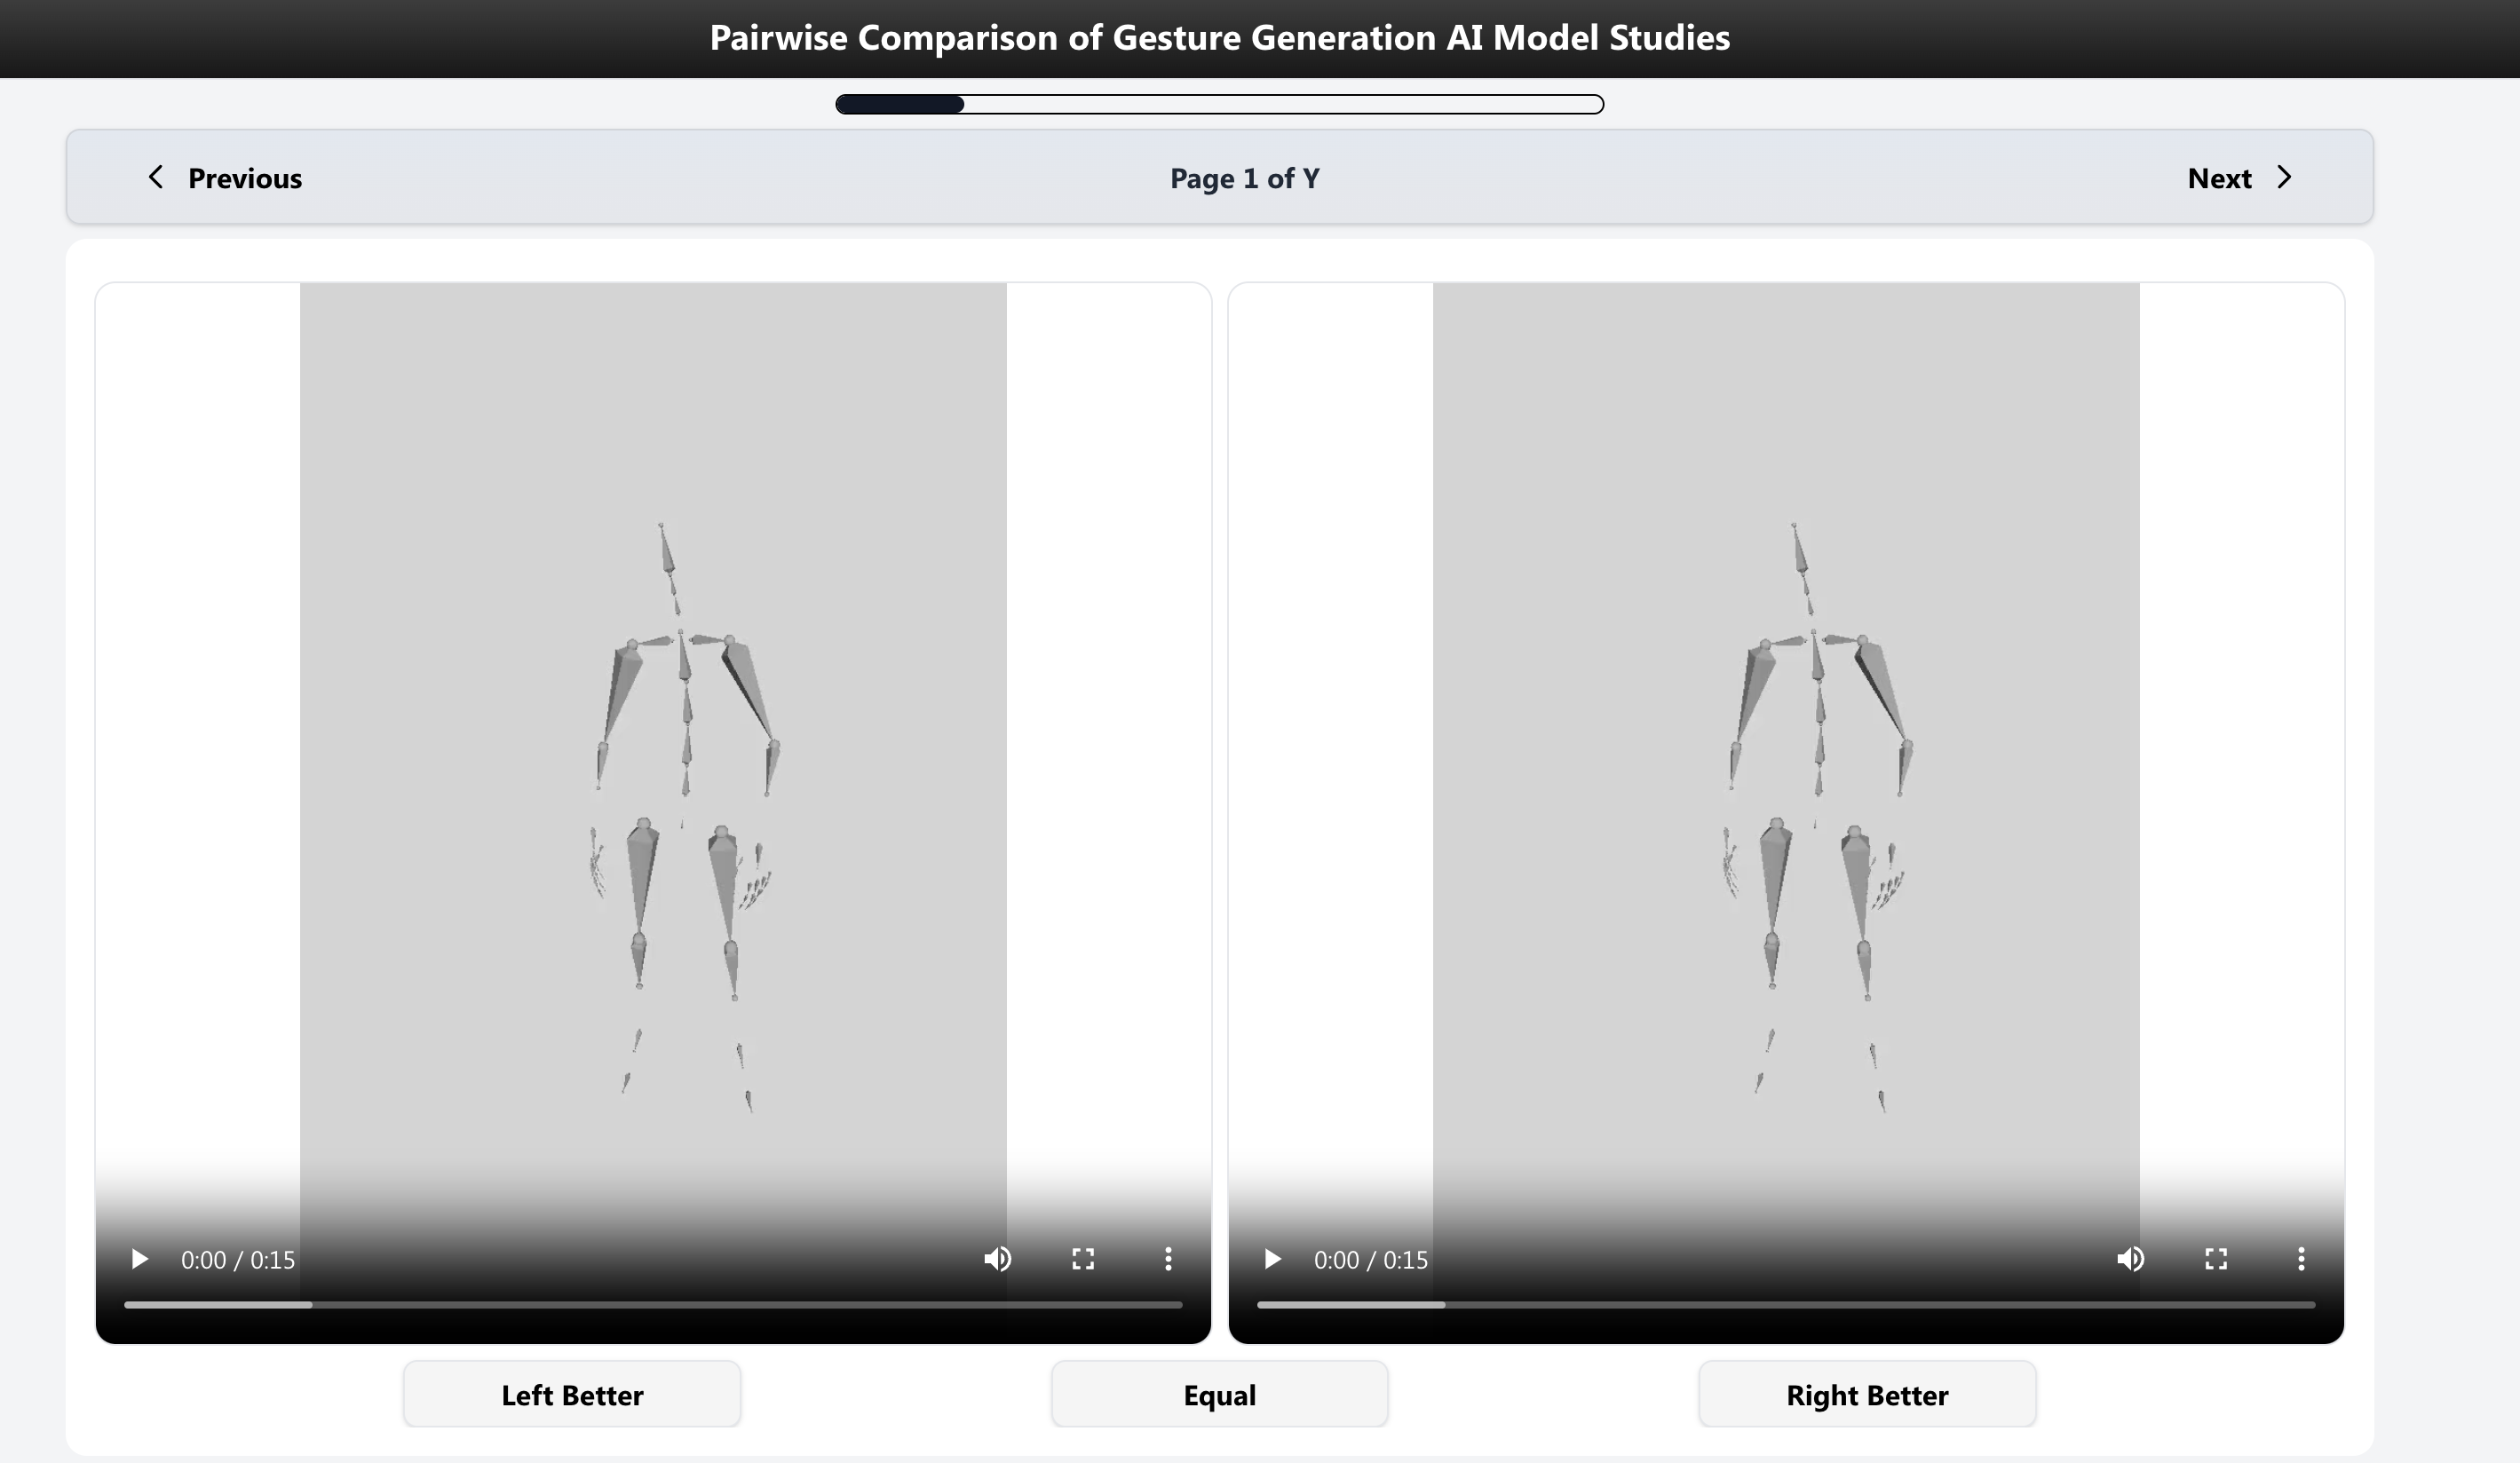
\includegraphics[width=\linewidth]{images/hemvip}
%	\caption{HEMVIP system used to evaluate rendering results of two models}
%	\Description{HEMVIP system used to evaluate rendering results of two models}
%\end{figure}

Within the GENEA group (\textbf{G}eneration and \textbf{E}valuation of \textbf{N}on-verbal Behaviour for \textbf{E}mbodied \textbf{A}gents), we hire evaluators on Prolific and conduct a user study based on the rendered video results. Participants rate the results as \textit{Left Better}, \textit{Equal}, or \textit{Right Better}. The updated scores are $-1$, $0$, and $1$ for each model, including ground truth data. The comparative results for all models are updated using the Elo rating system.

The source code is available at \hyperlink{https://github.com/hemvip/hemvip.github.io/}{github.com/hemvip.github.io}
\footnote{HEMVIP 2 \url{https://github.com/hemvip/hemvip.github.io}}.

\subsubsection{Evaluation Based on Quantitative Metrics}

\textbf{Mean Square Error (MSE)}

The mean square error between the predicted gesture sequence $\hat{\mathbf{y}}_i^{1:M \times D}$ and the ground-truth gesture sequence $\mathbf{y}_i^{1:M \times D}$ is computed as follows:

\begin{equation}
	\text{MSE} = \frac{1}{n} \sum_{i=1}^n \left\| \mathbf{y}_i^{1:M \times D} - \hat{\mathbf{y}}_i^{1:M \times D} \right\|^2
\end{equation}

Where:
\begin{itemize}
	\item $n$ is the number of data samples.
	\item $\mathbf{y}_i^{1:M \times D}$ is the ground truth of the $i^{th}$ sample, with $M$ being the number of frames and $D$ the number of data dimensions.
	\item $\hat{\mathbf{y}}_i^{1:M \times D}$ is the predicted value of the $i^{th}$ sample, having the same size $M \times D$.
	\item $\left\| \mathbf{y}_i^{1:M \times D} - \hat{\mathbf{y}}_i^{1:M \times D} \right\|^2$ is the squared norm of the difference between the ground truth and the predicted matrix.
\end{itemize}

MSE measures the average squared difference between the actual and predicted gesture sequences. The smaller the value, the more accurate the model's predictions. Evaluation results are presented in \autoref{subsec:MSEResult}.

\textbf{Fréchet Gesture Distance (FGD)}

Similar to image generation methods that use the Fréchet Inception Distance (FID) to measure distributional differences between real and generated data, the Fréchet Gesture Distance (FGD) measures the similarity in distribution between generated gesture sequences $\hat{\mathbf{y}}_i^{1:M \times D}$ and real gesture sequences $\mathbf{y}_i^{1:M \times D}$:

\begin{equation}
	\text{FGD} = \left\| \hat{\mu} - \mu \right\|^2 + \operatorname{Tr}\left( \Sigma + \hat{\Sigma} - 2 \sqrt{\Sigma \hat{\Sigma}} \right)
	\label{eq:fidscore}
\end{equation}

Where $n$ is the number of samples, and the parameters are defined as:

\begin{itemize}
	\item $\mu = \frac{1}{n} \sum_{i=1}^n \mathbf{y}_i^{1:M \times D}$ and $\hat{\mu} = \frac{1}{n} \sum_{i=1}^n \hat{\mathbf{y}}_i^{1:M \times D}$ are the mean feature vectors of the real dataset $\mathbf{y}_i^{1:M \times D}$ and generated dataset $\hat{\mathbf{y}}_i^{1:M \times D}$, respectively.
	
	\item $\Sigma = \frac{1}{n-1} \sum_{i=1}^n \left( \mathbf{y}_i^{1:M \times D} - \mu \right) \left( \mathbf{y}_i^{1:M \times D} - \mu \right)^T$ and
	
	$\hat{\Sigma} = \frac{1}{n-1} \sum_{i=1}^n \left( \hat{\mathbf{y}}_i^{1:M \times D} - \hat{\mu} \right) \left( \hat{\mathbf{y}}_i^{1:M \times D} - \hat{\mu} \right)^T$ are the covariance matrices of the features from the real and generated datasets, respectively.
	
	\item $\operatorname{Tr}(\cdot)$ denotes the matrix trace operator, which sums the diagonal elements.
	
	\item $\sqrt{\Sigma \hat{\Sigma}}$ denotes the matrix square root of the product of the two covariance matrices.
\end{itemize}

A low FGD score indicates that the distribution of generated gestures is close to the real gestures, while a high FGD suggests a large distributional difference and therefore lower gesture generation quality. In this study, the evaluation is performed on the predicted gesture sequence $\hat{\mathbf{x}}^{0} \in \mathbb{R}^{1:M \times D}$ and the ground-truth gesture sequence $\mathbf{x}_{0} \in \mathbb{R}^{1:M \times D}$.

\subsection{Evaluation Results}
\label{sec:result}

\subsubsection{User Study Evaluation Results}

\textbf{MOS Evaluation Results}

This work reuses the evaluation results of the baseline model \textbf{DiffuseStyleGesture} \cite{yang2023diffusestylegesture} for human perception metrics, as gesture generation remains a nascent field and the cost of evaluating multiple models is high. Therefore, this paper does not include evaluation results for the proposed \textbf{OHGesture} model.

%\begin{figure}[htbp]
%	\centering
%	\begin{subfigure}[b]{0.3\linewidth}
%		\includegraphics[width=\linewidth]{images/BoxHumanLikeness.pdf}
%		\caption*{\footnotesize (a) Human-likeness}
%	\end{subfigure}
%	\hfill
%	\begin{subfigure}[b]{0.3\linewidth}
%		\includegraphics[width=\linewidth]{images/BoxSpeechAppropriateness.pdf}
%		\caption*{\footnotesize (b) Speech Appropriateness}
%	\end{subfigure}
%	\hfill
%	\begin{subfigure}[b]{0.3\linewidth}
%		\includegraphics[width=\linewidth]{images/BoxStyleAppropriateness.pdf}
%		\caption*{\footnotesize(c) Style Appropriateness}
%	\end{subfigure}
%	\label{fig:compare}
%\end{figure}

To understand the visual performance of the proposed method, this paper conducts a user study comparing gestures generated by the proposed method with those from real motion capture data. The duration of the evaluated video clips ranges from 11 to 51 seconds, with an average length of 31.6 seconds — longer than clips used in the GENEA evaluation \cite{yoon2022genea} (8–10 seconds), as longer durations can provide clearer and more convincing results \cite{yang2022reprgesture}. Participants rated each video on a scale from 5 to 1, labeled $\texttt{excellent}$, $\texttt{good}$, $\texttt{fair}$, $\texttt{poor}$, and $\texttt{bad}$. 

\begin{table}[h]
	\centering
	\begin{tabular}{lcc}
		\hline
		\multicolumn{1}{c}{Name} &
		\begin{tabular}[c]{@{}c@{}}Human\\ likeness \end{tabular}$\uparrow$ &
		\begin{tabular}[c]{@{}c@{}}Gesture-speech\\ appropriateness\end{tabular}$\uparrow$ \\ \hline
		Ground Truth          & 4.15 $\pm$ 0.11          & 4.25 $\pm$ 0.09          \\
		Ours                  & \textbf{4.11 $\pm$ 0.08} & \textbf{4.11 $\pm$ 0.10} \\
%		\quad$-$ WavLM             & 4.05 $\pm$ 0.10          & 3.91 $\pm$ 0.11          \\
%		\quad$-$ Cross-local attention   & 3.76 $\pm$ 0.09          & 3.51 $\pm$ 0.15          \\
%		\quad$-$ Self-attention    & 3.55 $\pm$ 0.13          & 3.08 $\pm$ 0.10          \\
%		\quad$-$ Attention + GRU&
%		3.10 $\pm$ 0.11 &
%		2.98 $\pm$ 0.14 \\
%		\quad$+$ Forward attention & 3.75 $\pm$ 0.15          & 3.23 $\pm$ 0.24          \\
		\hline
	\end{tabular}
	\caption{Evaluation results using MOS}
	\label{table:MOSScore}
\end{table}
% Results of the ablation studies. "$-$" indicates removed modules, "$+$" indicates added modules. Bold indicates best performance.

\subsubsection{Quantitative Evaluation Results}

\textbf{Evaluation Results using MSE}
\label{subsec:MSEResult}

In this study, the predicted gesture sequence is segmented over $M$ frames. Mean Square Error (MSE) is applied to the gesture sequence $\mathbf{x}^{1:M \times D}$.

\begin{table}[h]
	\centering
	\resizebox{\linewidth}{!}{%
		\begin{tabular}{lcccccc}
			\hline
			\multicolumn{1}{c}{Emotion} & Neutral & Sad & Happy & Relaxed & Elderly & Angry \\ \hline
			DiffuseStyleGesture  & 75.04 & 51.40 & 110.18 & 130.83     & 116.03    & 78.53     \\
			ZeroEGG & 136.33 & 81.22 & 290.47 & 140.24     & 102.44    & 181.07     \\
			\hline
			Proposed Model                     &         &         &         &           &          &                 \\
			\quad \textbf{OHGesture} & 161.22 & 89.58 & 279.95 & 156.93   & 99.86   & 215.24    \\
			\hline
		\end{tabular}%
	}
	\caption{Mean Square Error results across 6 emotion categories}
	\label{table:EvaluationMSE}
\end{table}

\textbf{Evaluation Results using FGD}

This work proposes Fréchet Gesture Distance (FGD), a gesture-based variant of FID, and develops the open-source tool \hyperlink{https://github.com/GestureScore/GestureScore}{GestureScore} \footnote{Github/GestureScore: \url{https://github.com/GestureScore/GestureScore}}. In GestureScore, an Inception V3 model is implemented to encode the frame sequence $\bx^{1:M \times D}$ into a latent feature vector of size $32 \times 32$, which is then used as input to \autoref{eq:fidscore}. The following \autoref{table:EvalFGD} shows the FGD evaluation results of the OHGesture model using GestureScore.

%\begin{table}[h]
%	\centering
%	\begin{tabular}{lcc}
%		\hline
%		\multicolumn{1}{c}{Name} & FGD on Feature Vectors & \begin{tabular}[c]{@{}c@{}} FGD on Raw Data \end{tabular} \\ \hline
%		Ground Truth             & -       & -          \\
%		Ours                     &       & \\
%		\quad OHGesture (Feature D=1141) & 2.058      & 9465.546 \\
%		\quad OHGesture (Rotations) & 3.513       & 9519.129 \\
%		\hline
%	\end{tabular}
%	\caption{Evaluation results of Fréchet Gesture Distance (FGD) on $\bx^{1:M \times D}$ (from frame 1 to frame M, with D features per frame)}
%	\label{table:EvalFGD}
%\end{table}

\begin{table}[h]
	\centering
	\resizebox{\linewidth}{!}{
		\begin{tabular}{lcc}
			\hline
			\multicolumn{1}{c}{Name} & FGD on Feature Vectors & FGD on Raw Data \\ \hline
			Ground Truth             & -             & -            \\
			Ours                     &               &              \\
			\quad OHGesture (Feature D=1141) & 2.058  & 9465.546     \\
			\quad OHGesture (Rotations)      & 3.513  & 9519.129     \\
			\hline
		\end{tabular}
	}
	\caption{Evaluation results of Fréchet Gesture Distance (FGD) on $\bx^{1:M \times D}$ (from frame 1 to frame M, with D features per frame)}
	\label{table:EvalFGD}
\end{table}

\begin{itemize}
	\item \textbf{Feature Vectors:} The BVH files are used to convert the entire skeleton of each frame into a feature vector of size $D = 1141$, as described in \autoref{eq:gesturevector}.
	
	\item \textbf{Rotations:} From the resulting BVH file, this paper extracts the rotation angles, $D = 225$ ($225 = 75 \times 3$), from the gesture sequence of length $M$ frames for evaluation in the OHGesture row below.
\end{itemize}

\subsection{Building and Standardizing a Gesture Generation Evaluation System}

Currently, gesture generation is an active research area with many different models. However, there is no shared evaluation metric. Traditional metrics such as FID (Fréchet Inception Distance) or IS (Inception Score) fail to capture the human-likeness, speech appropriateness, and style appropriateness of generated gestures. Moreover, models are trained and evaluated on different datasets, making it difficult to compare results and determine which model is superior or state-of-the-art. This lack of a standardized evaluation protocol hampers progress in gesture generation research.

To address this, we proposes building an online leaderboard system \cite{nagy2024towards} \hyperlink{https://genea-workshop.github.io/leaderboard/}{GENEA Leaderboard} \footnote{GENEA Leaderboard: \url{https://genea-workshop.github.io/leaderboard/}}, which ranks gesture generation models. The thesis collects and processes gesture data from multiple languages and datasets, standardizes them into a unified dataset, and invites authors of various models to train and infer on this standardized set. The resulting generated gestures are then evaluated by hired participants through Prolific. 

The thesis is also building an online system \hyperlink{https://github.com/hemvip/hemvip.github.io}{hemvip/hemvip.github.io} \footnote{HEMVIP2 \url{https://github.com/hemvip/hemvip.github.io}} to support the evaluation process via Prolific-based crowd-sourcing. Evaluation results for the OHGesture model will be added based on this system.

Through this evaluation system, the research aims to establish a common benchmark, thereby fostering advancement in gesture generation.









% ********************** ********************** ********************** ********************** **********************


%
%
%
%In this section, we first introduce the setup of our system and then evaluate its performance, followed by quantitative and qualitative comparisons with other recent systems. Lastly, we do the ablation study to make an overall analysis of our system.
%
%\subsubsection{System Setup}
%\label{subsec:system_setup}
%\textbf{Datasets}
%\label{subsubsection:datasets}
%Three speech-gesture datasets are used in this paper: the Trinity dataset \cite{ferstl2018investigating}, the TED dataset \cite{yoon2019robots}, and a Chinese dataset collected for this work.
%
%Trinity Gesture dataset is a large database of speech and gestures jointly collected by \citet{ferstl2018investigating}. This dataset consists of $242$ minutes of motion capture and audio of one male actor talking on different topics. The actor’s motion was captured with a $20$-camera Vicon system and solved onto a skeleton with $69$ joints. In this paper, we use the official release version of \emph{The GENEA Challenge $2020$ Dataset} \cite{kucherenko2021large}, where $221$ minutes are used as training data, and the remaining $21$ minutes are kept for testing.
%
%TED Gesture dataset \cite{yoon2019robots} is a 3D upper-body gesture dataset collected using 3D pose estimation from English TED videos. This dataset includes 3D upper-body gestures of the speakers, the aligned speech audios, and text transcripts. In total, there are $253,186$ data samples, $80\%$ of which are training samples, $10\%$ belong to the validation set, and the remaining $10\%$ are test samples. The duration of each data sample is $34$ frames at a rate of $15$ fps, so the total length of this dataset is about $97$ hours. Notably, we adapt our model to take 3D joint positions instead of rotations for the TED dataset. The generated gestures are also represented in 3D joint positions, which are then converted into joint rotations for visualization.
%
%Additionally, we collected a $4$-hours ($80\%$ are the training data and $20\%$ are used for testing) Chinese Gesture dataset using the Noitom Perception Neuron Pro system. This dataset contains 3D full-body gestures of five speakers, aligned speech audios, and Chinese text transcripts. The text transcripts were recognized by Alibaba Cloud Automatic Speech Recognition (ASR) service. The skeleton of this dataset is retargeted to be consistent with the Trinity Gesture dataset. To ensure semantic richness, speakers are instructed to cover a diverse set of topics, such as cooking, fiction, philosophy of life, and academic reporting. \fig\ref{fig:onset_intervals_Chinese} illustrates the distribution of onset intervals in our dataset, and \fig\ref{fig:lexicon_tsne_Chinese} shows the visualization of the learned gesture lexicon on our dataset.
%
%\textbf{System Settings}
%All the motion data are downsampled to $20$, $20$, and $15$ frames per second on the Trinity, Chinese, and TED datasets, respectively. The range of onset intervals $[D_m, D_M]$ is $[0.2s,$ $0.5s]$ for both the Trinity and TED datasets, but $[0.3s, 0.6s]$ for the Chinese dataset. The length of each normalized block $K$ $=$ $\lceil D_M\times{}fps \rceil$. The generator synthesizes $4$ seconds of gestures at a time. The dimensions of $d_t$, $d_{\tilde{a}}$, $d_{\tilde{A}}$, $d_{\tilde{m}}$, $d_s$, $d_z$, and $d_{P}$ are $768$, $128$, $128$, $128$, $192$, $32$, and $32$ respectively. The size of the gesture lexicon $N_s$ is $50$ for both the Trinity and Chinese datasets but $100$ for the TED dataset. We train our framework using the Adam optimizer with $\beta1 = 0.9$, $\beta2 = 0.999$ and a learning rate of $0.0003$. The loss weights $w_{\alpha}, w_{\beta}$, $w_{\eqword{rec}}$, $w_{\eqword{perc}}$, $w_{\eqword{lexeme}}$, and $w_{{z}}$ are set as $1.0$, $1.0$, $1.0$, $0.5$, $0.2$, and $1.0$, respectively. At runtime, we use a Gaussian filter with a kernel size of $K$ to smooth the denormalized gesture sequence, where $K=5$ is chosen to generate the results presented in this paper.
%
%We train separate gesture generators on the Trinity, TED, and Chinese datasets. The cross-language capability of a generator can be further enhanced by pre-training the audio encoder (Section \ref{subsubsec:audio_representation}) using datasets in different languages. We have tried pre-training the audio encoder using both an English dataset (such as the Trinity or TED datasets) and our Chinese dataset and using it to train the generator on the Chinese dataset only. The gesture results can be found in the supplementary video.
%
%\begin{figure*}[t]
%    \centering
%    \includegraphics[width=\textwidth]{figures/fig6.pdf}
%    \caption{Qualitative results on the gestures synthesized by our method for four sample speech excerpts from the Trinity Gesture dataset \cite{ferstl2018investigating}. The character makes a metaphoric gesture when saying \emph{fine} and an iconic gesture for \emph{defend}. There are beat gestures for the words like \emph{thing} and \emph{selling}, and a deictic gesture appears when the character says \emph{me}. The drawing of this figure is inspired by \cite{yoon2020speech}.}
%    \Description{}
%    \label{fig:fig6}
%\end{figure*}
%
%\begin{figure*}[t]
%    \centering
%    \begin{subfigure}[t]{\textwidth}
%        \centering
%        \includegraphics[width=\textwidth]{figures/fig7a.pdf}
%        \caption{Low right hand, middle right hand, high right hand and time series statistics of right-hand height editing.}
%        \label{fig:fig7a}
%    \end{subfigure}
%    \begin{subfigure}[t]{\textwidth}
%        \centering
%        \includegraphics[width=\textwidth]{figures/fig7b.pdf}
%        \caption{Low average speed, middle average speed, high average speed and time series statistics of speed editing.}
%        \label{fig:fig7b}
%    \end{subfigure}
%    \begin{subfigure}[t]{\textwidth}
%        \centering
%        \includegraphics[width=\textwidth]{figures/fig7c.pdf}
%        \caption{Low average radius, middle average radius, high average radius and time series statistics of radius editing.}
%        \label{fig:fig7c}
%    \end{subfigure}
%    \caption{Results of style editing for the right-hand height (the first row), the hand speed (the second row), and the hand radius (the third row). The graphs on the right show the editing input (flat line) and the corresponding values of the output motions. The box plots show the statistics of the output.}
%    \label{fig:fig7}
%    \Description{}
%\end{figure*}
%
%\subsubsection{Evaluation}
%\label{subsec:evaluation}
%Figure \ref{fig:fig6} shows the gesture synthesis results for the speech excerpts from the test set of the Trinity dataset. Our system generates different types of realistic gestures. The character makes a metaphoric gesture when saying \emph{fine} and an iconic gesture for \emph{defend}. There are beat gestures for words like \emph{thing} and \emph{selling}, and a deictic gesture appears when the character says \emph{me}.
%
%We also did a cross-language synthesis experiment to test the robustness of our system. We use the pre-trained model trained on the Trinity dataset (an English dataset) to generate gestures for a Chinese speech clip. Since different languages do not share the same word embedding, we generate gestures by taking only the speech audio as input (Section \ref{subsec:inference_based_on_audio_only}). As illustrated in Figure \ref{fig:fig9b}, when encountering a different language, our system still generates beat-matched and stylized gestures, reflecting the robustness of our system. We also trained our system on the Chinese dataset and then did another cross-language experiment by generating gestures for an English speech excerpt. Please refer to the supplementary video for the visualization results.
%
%\textbf{Style Editing}
%\label{subsubsec:style_editing}
%Inspired by the idea of \citet{alexanderson2020style}, we augment our system to achieve motion editing by adding a feature block $\vect{C} \in\mathbb{R}^{K\times{}d_{c}}$ of the gesture motion as an extra input of the generator and the lexeme interpreter (\fig\ref{fig:interpreters}). The computations in \eqn\eqref{eqn:generator_block} and \eqref{eqn:lex_interpreter} are then reformulated as
%\begin{align}
%    \vect{M}_{i}^* &=\mathcal{G}(\tildevect{M}_{i-1},\tildevect{A}_{i},\vect{s}_i,\vect{z}_i,\vect{P},\vect{C}_i), \\
%    \vect{s}_i^* &=\mathcal{P}_s(\vect{s}_{i-1}^*, \tildevect{A}_i^{\eqword{H}}, \tildevect{T}_i, \vect{I},\vect{C}_i), 
%\end{align}
%which allows the network to learn the relationship between a desired motion feature and a gesture motion. During inference phase, we can easily edit the motion style feature of the generated gestures by modifying the feature block $\vect{C}$ as needed.
%
%Similar to \cite{alexanderson2020style}, we have experimented with three different style features using our system: the height of the right-hand (hand height), the average speed of both hands (hand speed), and the average distance from the hand positions to the up-axis through the root joint of the character (hand radius). We train a separate generator for each style feature. The training data is computed using the reference motions and averaged within a four-second sliding window, forming $K$-frame feature blocks. 
%
%We have synthesized three animations for each of the motion styles. Each animation has a constant desired low, mid, or high feature value, as shown in the first three columns of \fig\ref{fig:fig7}. The last column of \fig\ref{fig:fig7} shows the accuracy of the generated motion features. These results indicate that all the editing signals could efficiently affect the generated gestures.
%
%\subsubsection{Comparisons}
%\label{sbusec:comparisons}
%In this section, we compare our system with several state-of-the-art systems to demonstrate the advances made by our system. We first briefly introduce these systems and then our quantitative and qualitative comparisons. We also propose a simple but effective objective metric (PMB) to evaluate the rhythm performance for co-speech gesture synthesis.
%
%\begin{table*}[t]
%    \centering
%    \caption{Comparison of our system to SG \cite{alexanderson2020style}, Ges \cite{kucherenko2020gesticulator}, GTC \cite{yoon2020speech}, and S2AG \cite{bhattacharya2021speech2affectivegestures} on the TED and Trinity datasets. The system without beat segmentation (w/o BC) uses a fixed interval of $D_M$ for segmentation, which is $0.5s\sim{}0.6s$ depending on which dataset is used. The system without gesture lexeme (w/o SC) excludes the gesture lexicon and lexeme interpreter modules. The generator is retrained to predict future gestures based on only the previous motion, the audio, and the style code. Similarly, the system without gesture style code (w/o ZC) excludes the style code and the style interpreter modules. Only the motion, the audio, and the lexeme are used by the generator. \emph{Ours (audio only)} denotes the audio-only inference.}
%    \label{tab:table1}
%    
%    \newcolumntype{Y}{>{\raggedleft\arraybackslash}X}
%    \newcolumntype{Z}{>{\centering\arraybackslash}X}
%    \begin{tabularx}{\linewidth}{XXYYYY}
%        \toprule
%        Dataset & System & MAJE ($mm$) $\downarrow$ & MAD ($mm/s^2$) $\downarrow$ & FGD $\downarrow$ & PMB ($\%$) $\uparrow$ \\
%        \toprule
%        \multirow{8}*{Trinity} & Real Gesture & 0.0 & 0.0 & - & 95.74 \\
%        \cline{2-6}
%        & SG & 97.29 & 4.26 & 36.98 & 54.54 \\
%        & Ges & 82.41 & 3.62 & 31.04 & 71.0 \\
%        & S2AG & 54.93 & 1.49 & 20.36 & 79.53 \\
%        \cline{2-6}
%        & Ours (w/o BC) & 59.11 & 1.89 & 16.13 & 78.18 \\
%        & Ours (w/o SC) & 70.10 & 2.51 & 29.75 & 85.74 \\
%        & Ours (w/o ZC) & 52.85 & 1.35 & 12.53 & $\bm{91.36}$ \\
%        & Ours (audio only) & 57.99 & 1.83 & 15.79 & 87.35 \\
%        & Ours & $\bm{49.53}$ & $\bm{0.97}$ & $\bm{10.78}$ & $\bm{91.36}$ \\
%        
%        \midrule
%        \multirow{7}*{TED} & Real Gesture & 0.0 & 0.0 & - & 93.10 \\
%        \cline{2-6}
%        & GTC & 26.95 & 3.03 & 3.73 & 71.72 \\
%        & S2AG & 24.49 & 2.93 & 3.54 & 75.57 \\
%        \cline{2-6}
%        & Ours (w/o BC) & 27.10 & 3.11 & 3.88 & 67.88 \\
%        & Ours (w/o SC) & 30.07 & 3.53 & 5.22 & 83.10 \\
%        & Ours (w/o ZC) & 21.33 & 2.61 & 2.47 & 88.67 \\
%        & Ours (audio only) & 27.28 & 3.17 & 3.96 & 81.33 \\
%        & Ours & $\bm{18.13}$ & $\bm{2.29}$ & $\bm{2.04}$ & $\bm{89.52}$ \\
%        \bottomrule
%    \end{tabularx}
%    
%\end{table*}
%
%\begin{figure}[t]
%    \centering
%    \begin{subfigure}[t]{0.47\linewidth}
%        \centering
%        \includegraphics[width=\linewidth]{figures/table1a.pdf}
%        \caption{Trinity Gesture Dataset}
%        \label{fig:table1a}
%    \end{subfigure}
%    \hspace{\fill}
%    \begin{subfigure}[t]{0.47\linewidth}
%        \centering
%        \includegraphics[width=\linewidth]{figures/table1b.pdf}
%        \caption{TED Gesture dataset}
%        \label{fig:table1b}
%    \end{subfigure}
%    \Description{}
%    \caption{PMB results of continuously adjusting the threshold $\delta$ on the Trinity and TED datasets.}
%    \label{fig:table1}
%\end{figure}
%
%\textbf{Systems of Comparison}
%We choose four recent successful 3D co-speech gesture synthesis systems for comparison. On the Trinity dataset, we compare with the systems of Style Gesture (SG) \cite{alexanderson2020style} and Gesticulator (Ges) \cite{kucherenko2020gesticulator}. SG generates gestures based on only the speech audio and uses a normalizing flow model. Ges leverages the audio and text of the speech to generate semantically consistent gestures. On the TED dataset, we compare the systems of Gestures from Trimodal Context (GTC) \cite{yoon2020speech} and Speech to Affective Gestures (S2AG) \cite{bhattacharya2021speech2affectivegestures}. GTC uses speech audio, text transcript, and speaker identity to generate gestures. Based on the three modalities used in GTC, S2AG adds another new modality of affective expressions from the seed poses into their model.
%
%Because we have no access to the official pretrained model of SG, we strictly follow the official configuration and run the codes offered by authors to train a model. For other systems, we use the pretrained models provided by the authors. For a fair comparison, we use the same skeleton and motion frame rate as the baselines.
%
%\textbf{Quantitative Evaluation}
%
%\begin{figure*}[t]
%    \centering
%    \begin{subfigure}[t]{0.48\textwidth}
%        \centering
%        \includegraphics[width=\textwidth]{figures/fig8a.pdf}
%        \caption{Mean ratings for the English speech clips.}
%        \label{fig:fig8a}
%    \end{subfigure}
%    \hspace{\fill}
%    \begin{subfigure}[t]{0.48\textwidth}
%        \centering
%        \includegraphics[width=\textwidth]{figures/fig8b.pdf}
%        \caption{Mean ratings for the Chinese speech clips.}
%        \label{fig:fig8b}
%    \end{subfigure}
%    \caption{User study results with $95\%$ confidence intervals. Asterisks indicate the significant effects ($*: p < 0.05$, $**: p < 0.01$, $***: p < 0.001$). All the models are trained on the Trinity dataset (an English dataset). See Section \ref{subsubsec:user_study} for details.}
%    \Description{}
%    \label{fig:fig8}
%\end{figure*}
%
%We first adopt three commonly used evaluation metrics (MAJE, MAD, and FGD) to compare these systems quantitatively. 
%MAJE measures the \textbf{m}ean of the \textbf{a}bsolute \textbf{e}rrors between the generated \textbf{j}oint positions and the ground truth over all the time steps and joints, which indicates how closely the generated joint positions follow the ground truth. 
%MAD measures the \textbf{m}ean of the $\ell_2$ norm \textbf{d}ifferences between the generated joint \textbf{a}ccelerations and the ground truth over all the time steps and joints, which indicates how closely the ground truth and the generated joint movements match.
%\textbf{F}r{\'e}chet \textbf{G}esture \textbf{D}istance (FGD) was proposed by \citet{yoon2020speech}, which measures the difference between the distributions of the latent features of the generated gestures and ground truth, where the latent features are extracted using an auto-encoder trained on the Human 3.6M dataset \cite{ionescu2013human3}. FGD could assess the perceived plausibility of the synthesized gestures.  
%
%Calculating the matching rate between audio and motion beats is a standard method of evaluating rhythm performance, which has been widely used in music-driven dance synthesis \cite{Li_2021_aist, chen2021choreomaster}. However, we cannot simply apply this method to the gesture generation task because the onset of beat gesture usually precedes the corresponding speech beat by a small amount of time \cite{pouw2019quantifying}. Thus, we need a distance threshold to determine robustly whether the audio and motion beats match each other. 
%
%\textbf{P}ercentage of \textbf{c}orrectly predicted \textbf{k}eypoints (PCK)  is a widely used metric in human pose estimation \cite{Wei_2016_openpose, mehta2017vnect}, where a predicted key point is considered correct if its distance to the ground truth is smaller than an adjustable threshold. Inspired by this metric, we propose a new metric, \emph{PMB}, as the \textbf{p}ercentage of \textbf{m}atched \textbf{b}eats, where a motion beat is considered to be matched if its temporal distance to a nearby audio beat is smaller than a threshold $\delta$. Specifically,
%\begin{equation}
%    \eqword{PMB}(\vect{B}^{{m}}, \vect{B}^{{a}}) = \frac{1}{N_m}\sum^{N_m}_{i=1}\sum^{N_a}_{j=j_{[i-1]}^{{a}*}+1} \mathbbm{1}\big[\lVert \vect{b}_i^{{m}} - \vect{b}_j^{{a}} \rVert_1 < \delta\big].
%\end{equation}
%The sequence of motion beats $\vect{B}^{{m}}=\{\vect{b}_1^{{m}}, \dots, \vect{b}_{N_m}^{{m}}\}$, where $N_m$ is the number of motion beats, is identified using the algorithm proposed by \citet{ho2013motionbeat} based on the local minima of joint deceleration. 
%The audio beats $\vect{B}^{{a}}=\{\vect{b}_1^{{a}}, \dots, \vect{b}_{N_a}^{{a}}\}$ are the onset sequence, where $N_a$ is the number of onsets. $j_{[i-1]}^{{a}*}$ represents the index of the audio beats that the last motion beat matches. $\mathbbm{1}$ denotes the indicator function. The threshold $\delta$ is set to $0.2$s by default, but we can adjust $\delta$ continuously and observe the changes of the PMB values, which provides a more comprehensive picture of the rhythmic performance.
%
%Table \ref{tab:table1} summarizes the performance of all the systems on the two English datasets, Trinity and TED. For the MAJE, MAD, and FGD metrics, our system achieves the lowest values on both datasets. Note that the FGD values of our system are significantly lower than other systems, which indicates the better perceptual quality of gestures synthesized by our system. It is interesting that the FGD values rise rapidly without the gesture lexeme component (w/o SC), which means the gesture lexeme is crucial to gesture quality. There is a decline in the generation performance in the audio-only inference because of the lack of sufficient input information. However, the generated gestures are still acceptable.
%
%As for the rhythm performance, our system achieves the highest PMB values on both datasets. The PMB values drop rapidly without the beat segmentation component (w/o BC), indicating that beat segmentation is vital to rhythm awareness. Figure \ref{fig:table1} shows the PMB results with different thresholds. It can be seen that even the ground-truth motion does not match the speech beats precisely, while the behavior of our method is closer to the ground truth compared  with the baselines.
%
%\begin{figure*}[t]
%    \centering
%    \begin{subfigure}[t]{0.48\textwidth}
%        \centering
%        \includegraphics[width=\textwidth]{figures/fig9a.pdf}
%        \caption{Gesture results for an English speech clip.}
%        \label{fig:fig9a}
%    \end{subfigure}
%    \hspace{\fill}
%    \begin{subfigure}[t]{0.48\textwidth}
%        \centering
%        \includegraphics[width=\textwidth]{figures/fig9b.pdf}
%        \caption{Gesture results for a Chinese speech clip.}
%        \label{fig:fig9b}
%    \end{subfigure}
%    \caption{Generated motions of SG, Ges, and our system for the same input speech used in the user study. All the models are trained on the Trinity dataset (an English dataset). The red words indicate beats. The red arrows show the movement of corresponding beat gestures. A green check indicates a correct beat match, while a red cross indicates a wrong beat match.}
%    \label{fig:fig9}
%    \Description{}
%\end{figure*}
%
%\textbf{User Study}
%\label{subsubsec:user_study}
%We further conduct user studies to assess the performance of our system qualitatively, where SG \cite{alexanderson2020style} and Ges \cite{kucherenko2020gesticulator} are used as the baseline methods. 
%We generate $14$ test video clips, each consisting of the results synthesized by our methods, the baselines, and the ground truth in random order. Among the $14$ clips, nine are English clips generated from the test set of the Trinity dataset, and five are Chinese clips generated from the test set of our Chinese dataset. Notably, all the clips are synthesized using the models trained on the English Trinity dataset. The duration of each clip is around $30$s. 
%
%We have recruited $30$ volunteer participants to participate in our study, of which $19$ are male and $11$ are female. 19 participants are $18-22$ years of age, 10 are between $23-30$, and one is above $30$. When participants watch each video clip, they will be asked to answer three questions and rate the video from $1$ to $5$, with $1$ being the worst, $3$ being average, and 5 being the best. The three questions are: (1) human likeness (neglecting the speech audio), (2) speech-to-gesture content matching, and (3) speech-to-gesture beat matching. 
%
%The results of these user studies are shown in \fig\ref{fig:fig8}, our system receives higher scores than the other systems and is closer to the real gestures (GT). A one-way ANOVA reveals main effects of \emph{human likeness}, \emph{content matching}, and \emph{beat matching}, and a post-hoc Tukey multiple comparison test identifies a significant difference ($p < 0.005$) between our system and all the other methods. 
%%
%As also illustrated in \fig\ref{fig:fig9a}, the end-to-end systems SG and Ges are less sensitive to rhythm than ours, and the resulting motions lack diversity, which affects their performance in the user studies.
%
%The statistical results of the cross-language test (\fig\ref{fig:fig8b}) demonstrate the better robustness of our system. When dealing with a completely different language (\fig\ref{fig:fig9b}), the gestures generated by SG are more rigid and do not match the beats correctly. In contrast, our model (audio-only) is still able to perceive beats accurately and generate dynamic gestures. Notably, we do not compare with Ges in this cross-language test because this model only supports English text transcripts. 
%
%\subsubsection{Ablation Study}
%\label{subsec:ablation_study}
%We conduct a variety of ablation studies to analyze the performance of our system. Notably, only the ablation of the lexicon size (\fig\ref{fig:fig12}) uses the validation set of the dataset to determine the hyperparameter of the model. All other experiments are based on the test set.
%
%\textbf{Hierarchical Audio Feature Disentanglement}
%\label{subsubsec:disentanglement}
%We presume that the high-level audio feature $\vect{a}^{\eqword{high}}$ contains semantics-relevant information that determines the gesture lexeme $\vect{s}$.
%To justify this assumption, we apply the K-means algorithm to all the high-level audio blocks of the TED Gesture dataset and get 50 clusters, where each cluster essentially indexes the audio clips with similar semantics. We can find several representative clusters $\vect{C}^{\eqword{high}}_0$ whose corresponding text transcripts contain words with a similar meaning, such as \emph{many}, \emph{quite a few}, \emph{lots of}, \emph{much}, and \emph{more}, etc. Meanwhile, these audio clips also correspond to a set of generated motion blocks $\{\vect{M}^*_0,\vect{M}^*_1,\dots\}$. By encoding these motion blocks using the pre-trained encoder $\mathcal{E}$, we can obtain their corresponding motion latent codes. As illustrated in \fig\ref{fig:fig14a}, these latent codes (gray dots) only appear in a few gesture lexemes (orange, purple, and red), and it can be seen that the sample gestures of these latent codes indeed convey the semantics of the cluster $\vect{C}^{\eqword{high}}_0$.
%The same observation is not true for the low-level audio features. If we also cluster all low-level audio features and pick a representative cluster $\vect{C}^{\eqword{low}}_0$, \fig\ref{fig:fig14b} shows that the corresponding motion latent codes (various color dots) appear nearly uniformly in most of the gesture lexemes.
%The experiments above confirm the correlation between the high-level audio features and the gesture lexemes, as well as the semantic disentanglement between high-level and low-level audio features.
%
%\begin{figure}[t]
%    \centering
%    \begin{subfigure}[t]{0.62\linewidth}
%        \centering
%        \includegraphics[width=\linewidth]{figures/fig14a.pdf}
%        \caption{High-level}
%        \label{fig:fig14a}
%    \end{subfigure} 
%    \hspace{\fill}
%    \begin{subfigure}[t]{0.3554\linewidth}
%        \centering
%        \includegraphics[width=\linewidth]{figures/fig14b.pdf}
%        \caption{Low-level}
%        \label{fig:fig14b}
%    \end{subfigure} 
%    \caption{t-SNE visualization of motion latent codes. Each color (except gray) stands for a gesture lexeme. 
%    (a) latent codes (gray dots) corresponding to cluster $\vect{C}^{\eqword{high}}_0$ only appear in specific gesture lexemes (orange, purple, and red).
%    (b) latent codes (various color dots) corresponding to cluster $\vect{C}^{\eqword{low}}_0$ are distributed in most of the gesture lexemes.
%    See Section \ref{subsubsec:disentanglement} for details.}
%    \label{fig:fig14}
%    \Description{}
%\end{figure}
%
%\textbf{Gesture Style Code}
%\label{subsubsec:gesture_style_code}
%%
%\begin{figure}[t]
%    \centering
%    \begin{subfigure}[t]{0.32\linewidth}
%        \centering
%        \includegraphics[width=\linewidth]{figures/fig15a.pdf}
%        \caption{w/o $\vect{a}^{\eqword{low}},\vect{z}$}
%        \label{fig:fig15a}
%    \end{subfigure} 
%    \hspace{\fill}
%    \begin{subfigure}[t]{0.32\linewidth}
%        \centering
%        \includegraphics[width=\linewidth]{figures/fig15b.pdf}
%        \caption{w/ $\vect{a}^{\eqword{low}}$ + w/o $\vect{z}$}
%        \label{fig:fig15b}
%    \end{subfigure} 
%    \hspace{\fill}
%    \begin{subfigure}[t]{0.32\linewidth}
%        \centering
%        \includegraphics[width=\linewidth]{figures/fig15c.pdf}
%        \caption{w/ $\vect{a}^{\eqword{low}},\vect{z}$}
%        \label{fig:fig15c}
%    \end{subfigure} 
%    \caption{t-SNE visualization of real gestures (GT) versus generated gestures in the motion latent space. We randomly choose two gesture lemexes for visualization.
%    (a) results of our system without low-level audio feature and gesture style code.
%    (b) with low-level audio feature but without gesture style code.
%    (c) with low-level audio feature and gesture style code.
%    See Section \ref{subsubsec:disentanglement} for details.}
%    \label{fig:fig15}
%    \Description{}
%\end{figure}
%%
%\begin{table}[t]
%    \centering
%    \caption{Comparison of style interpreters w/ and w/o low-level audio features and gesture style code. See Section \ref{subsubsec:disentanglement} for details.}
%    \label{tab:table6}
%    
%    \begin{tabularx}{\linewidth}{lXrrr}
%        \toprule
%        Dataset & System & Variance $\uparrow$ & FGD $\downarrow$ & PMB ($\%$) $\uparrow$ \\
%        \toprule
%        \multirow{5}*{Trinity} & Real Gesture & 0.41 & - & 95.74 \\
%        \cline{2-5}
%        & w/o $\vect{a}^{\eqword{low}},\vect{z}$ & 0.09 & 17.99 & 89.35 \\
%        & w/ $\vect{a}^{\eqword{low}}$ + w/o $\vect{z}$ & 0.21 & 12.53 & $\bm{91.36}$ \\
%        & w/ $\vect{a}^{\eqword{low}},\vect{z}^{\eqword{random}}$ & 0.30 & 11.96 & 91.28 \\
%        & w/ $\vect{a}^{\eqword{low}},\vect{z}$ & $\bm{0.37}$ & $\bm{10.78}$ & $\bm{91.36}$ \\
%        
%        \midrule
%        \multirow{5}*{TED} & Real Gesture & 2.72 & - & 93.10 \\
%        \cline{2-5}
%        & w/o $\vect{a}^{\eqword{low}},\vect{z}$ & 0.89 & 3.71 & 84.57 \\
%        & w/ $\vect{a}^{\eqword{low}}$ + w/o $\vect{z}$ & 1.87 & 2.47 & 88.67 \\
%        & w/ $\vect{a}^{\eqword{low}},\vect{z}^{\eqword{random}}$ & $\bm{2.49}$ & 2.13 & 88.89 \\
%        & w/ $\vect{a}^{\eqword{low}},\vect{z}$ & 2.45 & $\bm{2.04}$ & $\bm{89.52}$ \\
%        \bottomrule
%    \end{tabularx}
%  
%\end{table}
%%
%\begin{table}[t]
%    \centering
%    \caption{Comparison of style interpreters w/ and w/o text features.}
%    \label{tab:table5}
%    
%    \newcolumntype{Y}{>{\raggedleft\arraybackslash}X}
%    \newcolumntype{Z}{>{\centering\arraybackslash}X}
%    \begin{tabularx}{\linewidth}{XlYY}
%        \toprule
%        Dataset & System & FGD $\downarrow$ & PMB ($\%$) $\uparrow$ \\
%        \toprule
%        \multirow{2}*{Trinity} & w/o text feature & 10.91 & $\bm{91.36}$ \\
%        & w/ text feature & $\bm{10.78}$ & $\bm{91.36}$ \\
%        
%        \midrule
%        \multirow{2}*{TED} & w/o text feature & 2.09 & 89.22 \\
%        & w/ text feature & $\bm{2.04}$ & $\bm{89.52}$ \\
%        \bottomrule
%    \end{tabularx}
%\end{table}
%%
%The low-level audio feature $\vect{a}^{\eqword{low}}$ contains semantic-irrelevant information, e.g., pitch and volume. Presumably, it should affect the motion variations within a gesture lexeme. In our system, we introduce the learnable gesture style code $\vect{z}$ combined with the low-level audio feature to jointly determine the motion variations, which can be considered a fine-grained style.
%As illustrated in Figure \ref{fig:fig15b}, the low-level audio feature increases the variety of the generated gestures but cannot fully decide the variations. With the introduction of the gesture style code (Figure \ref{fig:fig15c}), the distribution of generated gestures becomes closer to the ground-truth distribution. 
%
%Table \ref{tab:table6} compares several settings in terms of motion variance, FGD, and PMB. We measure the Euclidean distance from the motion latent code of a motion to the corresponding gesture lexeme and compute the variance of these distances corresponding to the same lexeme. The \emph{motion variance} is then defined as the average of such variances of every lexeme. $\vect{z}$ denotes the output of the style interpreter, while $\vect{z}^{\eqword{random}}$ is a random style code sampled from the normal distribution in the latent space. Consistent with Figure \ref{fig:fig15}, Table \ref{tab:table6} also shows that combining the low-level audio feature and styles achieves more significant motion variance and lower FGD values. Besides, the FGD values in Table \ref{tab:table6} also indicate that the style codes computed by the interpreter generate gestures that are more perceptually acceptable than that created using random style codes.
%
%We have also evaluated the importance of the text features in interpreting the gesture style codes (see \eqn\ref{eqn:style_interpreter}).
%The result of Table \ref{tab:table5} shows that interpreting the style codes 
%with text features does improve the FGD value. However, the improvement is marginal. Considering the inference efficiency, we can interpret the style codes conditional on only the low-level audio features.
%
%\textbf{Range of Onset Intervals}
%\label{subsubsec:onset_interval}
%Choosing a proper range of onset intervals is crucial to achieving quality gestures. Intuitively, the lower bound of this range affects the model's sensitivity to beat. If the lower bound is too high (such as 0.5s), the interval between the identified beats becomes large, causing the model to respond sluggishly to beats. The upper bound of the onset intervals regularizes the variance of the duration of the speech blocks, which should not be too large either. If the length of the speech blocks differs too much, the side effect of the normalization becomes visible, causing unnatural transitions between the generated gesture blocks. 
%
%To verify the above hypothesis, we compare the performance of three different interval ranges: 0.2-0.5s, 0.2-1.0s, and 0.5-1.0s, where 0.2-0.5s is our default setting (Section \ref{subsubsec:onset_identification}).
%As shown in Table \ref{tab:table2}, our default range of onset intervals achieves the best FGD and PMB values on both the Trinity and TED Gesture datasets. PMB drops significantly when the minimum distance between onsets is high (0.5-1.0s), which indicates that the model is insensitive to the rhythm. When the variance is too large (0.2-1.0s), PMB is barely affected, but FGD drops a lot, showing that the generated motions exhibit a lower quality. This result is consistent with our hypothesis.
%
%Moreover, to explicitly show the effect of the minimum onset interval, we visualize the synchronization between the motion and audio beats under different interval ranges in \fig\ref{fig:fig10}. 
%Similar to \citet{aristidou2021rhythm}, we calculate the motion beats based on the motion deceleration \cite{davis2018visual}.
%As shown in Figure \ref{fig:fig10}, the motion beats extracted under the interval range of 0.2-0.5s (denoted by the green stars) synchronize with the audio beats (dashed red lines). In contrast, the motion beats extracted under the interval range of 0.5-1.0s (denoted by the orange stars) do not match well with the audio beats, which proves that a high minimum interval (0.5s) will cause a low beat sensitivity of the model.
%
%\begin{table}[t]
%    \centering
%    \caption{Effects of the range of onset intervals.}
%    \label{tab:table2}
%    
%    \newcolumntype{Y}{>{\raggedleft\arraybackslash}X}
%    \newcolumntype{Z}{>{\centering\arraybackslash}X}
%    \begin{tabularx}{\linewidth}{XlYY}
%        \toprule
%        Dataset & Range of Onset Intervals & FGD $\downarrow$ & PMB ($\%$) $\uparrow$ \\
%        \toprule
%        \multirow{3}*{Trinity} & 0.5-1.0s & 25.45 & 73.87 \\
%        & 0.2-1.0s & 19.16 & 90.75 \\
%        & 0.2-0.5s & $\bm{10.78}$ & $\bm{91.36}$ \\
%        
%        \midrule
%        \multirow{3}*{TED} & 0.5-1.0s & 3.61 & 65.34 \\
%        & 0.2-1.0s & 2.55 & 89.10 \\
%        & 0.2-0.5s & $\bm{2.04}$ & $\bm{89.52}$ \\
%        \bottomrule
%    \end{tabularx}
%    
%\end{table}
%%
%\begin{figure}[t]
%    \centering
%    \includegraphics[width=\linewidth]{figures/fig10.pdf}
%    \caption{Audio-to-gesture synchronization under different ranges of onset interval. Motion beats are computed based on the local minima of joint deceleration. Audio beats are identified using the audio onsets.}
%    \label{fig:fig10}
%    \Description{}
%\end{figure}
%
%\begin{figure}[t]
%    \centering
%    \begin{subfigure}[t]{0.47\linewidth}
%        \centering
%        \includegraphics[width=\linewidth]{figures/fig11a.pdf}
%        \caption{w/ gesture lexeme}
%        \label{fig:fig11a}
%    \end{subfigure}
%    \hspace{\fill}
%    \begin{subfigure}[t]{0.47\linewidth}
%        \centering
%        \includegraphics[width=\linewidth]{figures/fig11b.pdf}
%        \caption{w/o gesture lexeme}
%        \label{fig:fig11b}
%    \end{subfigure}
%    \caption{t-SNE visualization of motion latent codes on the TED dataset, computed using the pre-trained encoder $\mathcal{E}$. Colors represent gesture lexemes.}
%    \label{fig:fig11}
%    \Description{}
%\end{figure}
%%
%\begin{table}[t]
%    \centering
%    \caption{Diversity of motions generated w/ and w/o gesture lexemes.}
%    \label{tab:table3}
%    
%    \newcolumntype{Y}{>{\raggedleft\arraybackslash}X}
%    \newcolumntype{Z}{>{\centering\arraybackslash}X}
%    \begin{tabularx}{\linewidth}{llY}
%        \toprule
%        Dataset & System & Diversity $\uparrow$ \\
%        \toprule
%        \multirow{3}*{Trinity} & Real Gesture & 3.79 \\
%        \cline{2-3}
%        & w/o gesture lexeme & 1.91 \\
%        & w/ gesture lexeme & $\bm{3.40}$ \\
%        
%        \midrule
%        \multirow{3}*{TED} & Real Gesture & 4.32 \\
%        \cline{2-3}
%        & w/o gesture lexeme & 2.99 \\
%        & w/ gesture lexeme & $\bm{4.09}$ \\
%        \bottomrule
%    \end{tabularx}
%
%\end{table}
%
%\textbf{Gesture Lexeme}
%\label{subsubsec:gesture_lexeme}
%Table \ref{tab:table1} has shown that FGD increases significantly without the gesture lexeme, indicating the importance of the gesture lexeme in achieving quality motions. Besides, as demonstrated in \fig\ref{fig:fig11}, the variety of the generated gestures is also significantly reduced without the gesture lexeme. To show this conclusion quantitatively, we calculate the entropy of the gesture lexemes to measure the motion diversity as
%\begin{equation}
%    \eqword{Diversity} = -\sum_{i=1}^{N_s}p_i\log{p_i},
%\end{equation}
%where $N_s$ is the size of gesture lexicon, $p_i$ indicates the occurrence frequency of the $i$-th lexeme in the generated gestures. As shown in Table \ref{tab:table3}, our system with the gesture lexeme creates much higher diversity than the system without it, which further testifies the conclusion of \fig\ref{fig:fig11} and again emphasizes the importance of the gesture lexeme.
%
%\textbf{Size of Gesture Lexicon}
%Figure \ref{fig:fig12} shows the performance of our system under different gesture lexicon sizes. It can be seen that neither too small nor too large lexicons achieve good results, measured as FGD values. On the one hand, a small gesture lexicon forces a diverse range of gesture motions to be merged into the same gesture lexeme, which aggravates the one-to-many mapping issue and causes the generator hard to learn all the motions. On the other hand, an excessively large lexicon forcibly splits many lexemes into sub-lexemes. These sub-lexemes are typically close together, making the gesture lexeme interpretation more challenging and thus negatively affecting the gesture quality. We note that the PMB metric is less affected by the gesture lexicon size, possibly because our beat-based segmentation and normalization mechanism explicitly enforces the gesture rhythm. Based on these experiments, we set the sizes of the gesture lexicon for the Trinity and TED dataset to 50 and 100, respectively, as shown in Figure \ref{fig:gesture_lexicon}.
%
%\begin{figure}[t]
%    \centering
%    \begin{subfigure}[t]{0.47\linewidth}
%        \centering
%        \caption*{Trinity Gesture dataset}
%        \includegraphics[width=\linewidth]{figures/fig12a.pdf}
%        \label{fig:fig12a}
%    \end{subfigure} 
%    \hspace{\fill}
%    \begin{subfigure}[t]{0.47\linewidth}
%        \centering
%        \caption*{TED Gesture dataset}
%        \includegraphics[width=\linewidth]{figures/fig12b.pdf}
%        \label{fig:fig12b}
%    \end{subfigure} 
%    \caption{Effects of the size of the gesture lexicon. The gray dashed lines mark the optimal lexicon size.}
%    \label{fig:fig12}
%    \Description{}
%\end{figure}
%%
%\textbf{Different Interpreters}
%%
%\begin{table}[t]
%    \centering
%    \caption{Comparison of interpreters. The statistical interpreter selects gesture lexemes based on the frequency distribution of lexemes but neglects the input speech. The learning-based interpreter is our default interpreter that translates the input speech into gesture lexemes.}
%    \label{tab:table4}
%    
%    \newcolumntype{Y}{>{\raggedleft\arraybackslash}X}
%    \newcolumntype{Z}{>{\centering\arraybackslash}X}
%    \begin{tabularx}{\linewidth}{XcYYY}
%        \toprule
%        \multirow{2}*{Dataset} & Interpreter  & Accuracy  & \multirow{2}*{FGD $\downarrow$} & PMB  \\
%        & Type &($\%$)         $\uparrow$ & & ($\%$) $\uparrow$\\
%        \toprule
%        \multirow{2}*{Trinity} & Statistical & 28.01 & 21.53 & 90.75 \\
%        & Learning-based & $\bm{59.15}$ & $\bm{10.78}$ & $\bm{91.36}$ \\
%        
%        \midrule
%        \multirow{2}*{TED} & Statistical & 32.11 & 3.57 & 87.99 \\
%        & Learning-based & $\bm{62.53}$ & $\bm{2.04}$ & $\bm{89.52}$ \\
%        \bottomrule
%    \end{tabularx}
%
%\end{table}
%
%In our system, the lexeme interpreter determines the sequence of gesture lexemes. Our learning-based interpreter described in Section~\ref{subsec:lexeme_interpreter} accomplishes this task according to the speech features and the previous lexemes. Besides, inspired by \cite{aristidou2021rhythm}, we further experiment with a statistical interpreter that matches the frequency of each lexeme in the generated gestures with the reference. Specifically, for a speaker~$\vect{I}$, we calculate the frequency distribution of gesture lexemes, $\vect{f}^{\vect{I}}\in\mathbb{R}^{N_s}$, and a transition matrix, $\vect{L}\in\mathbb{R}^{N_s\times{}N_s}$, describing the frequency of transitions between lexemes using the training data. These quantities can be considered as a global representation of speaker's gesture style. 
%%
%During inference, we configure the statistical interpreter to ensure that the lexeme distribution of the generated gesture sequence $\vect{f}_t$ matches the corresponding global distribution $\vect{f}^{\vect{I}}$. 
%%
%To achieve this goal, at each generation step, we compute a multinomial distribution characterized by $\vect{f}^*_{t+1}$ using the transition matrix and the difference between the current and target lexeme frequencies $\vect{f}_t$ and $\vect{f}_{\vect{I}}$, where
%\begin{equation}
%    \vect{f}^*_{t+1} = \softmax(\vect{f}^{\vect{I}}-\vect{f}_t )
%    \cdot \vect{L}.
%\end{equation}
%Then the next lexeme is sampled from the multinomial distribution.
%%
%This statistical interpreter does not consider the input speech but only the statistics of the generated gestures when selecting the lexemes. In practice, the result motions still look acceptable but more random. This can be confirmed by Table \ref{tab:table4}, where the statistical interpreter exhibits a lower prediction accuracy and higher FGD values than our learning-based method because of the lack of semantic information brought by the input speech.
%
%\textbf{Positional Encoding}
%\label{subsubsec:pos_enc}
%%
%\begin{table}[t]
%    \centering
%    \caption{Effects of the positional encoding block.}
%    \label{tab:pos_enc}
%    
%    \newcolumntype{Y}{>{\raggedleft\arraybackslash}X}
%    \newcolumntype{Z}{>{\centering\arraybackslash}X}
%    \begin{tabularx}{\linewidth}{XlYY}
%        \toprule
%        Dataset & System & FGD $\downarrow$ & PMB ($\%$) $\uparrow$ \\
%        \toprule
%        \multirow{2}*{Trinity} & w/o positional encoding & 11.15 & 89.98 \\
%        & w/ positional encoding & $\bm{10.78}$ & $\bm{91.36}$ \\
%        
%        \midrule
%        \multirow{2}*{TED} & w/o positional encoding & 2.19 & 88.13 \\
%        & w/ positional encoding & $\bm{2.04}$ & $\bm{89.52}$ \\
%        \bottomrule
%    \end{tabularx}
%\end{table}
%%
%The positional encoding block (\eqn\ref{eqn:pos_enc}) informs the generator about the frame-level progress of the synthesis in a motion block, which helps the generator model the temporal structure, especially the rhythm, of the sequence. As shown in Table \ref{tab:pos_enc}, the positional encoding block can improve the beat-matched rate (higher PMB) while enhancing the perceptual quality of generated movements (lower FGD).